\documentclass[12pt]{article}
\usepackage{amsmath, amssymb, amsfonts}
\usepackage[most]{tcolorbox}
\usepackage{lmodern}
\usepackage{fancyhdr}
\usepackage{multicol}
\usepackage{graphicx}
\usepackage{xcolor}
\usepackage{enumitem}

\definecolor{color1}{HTML}{941b0c}
\definecolor{color2}{HTML}{bc3908}
\definecolor{color3}{HTML}{f6aa1c}

\usepackage[font=small, labelfont=bf, justification=centering]{caption}
\usepackage[colorlinks=true, linkcolor=black, urlcolor=color2, citecolor=black]{hyperref}
\usepackage[a4paper, margin=1in]{geometry}

\title{\sffamily\bfseries{Soluções TM$^2$ 2023A}}
\author{Samuel de Araújo Brandão}
\date{2 de Agosto de 2025}

\renewcommand*\contentsname{\textsf{Contents}}

\pagestyle{fancy}
\fancyhf{}

\fancyhead[L]{\textbf{Soluções TM$^2$ 2023A}}
\fancyhead[R]{\textcolor{color2}{Samuel Brandão}, 2 de Agosto de 2025}
\fancyfoot[C]{\thepage}
\setlength{\headheight}{14.5pt}

\tcbset{
  problembox/.style={
    enhanced,
    colback=white,
    colframe=color2,
    boxrule=1pt,
    arc=2mm,
    top=1pt,
    bottom=1pt,
    left=1pt,
    right=1pt,
    fonttitle=\sffamily\bfseries\color{white},
    colbacktitle=color2,
    title={#1}
  }
}

\begin{document}
  \maketitle

  Uma coleção de soluções para a TM$^2$ 2024 nível A, inspirada no estilo de Evan Chen.

  Todas as soluções foram inteiramente escritas por mim, enquanto me preparava para a
  International Mathematical Olympiad (IMO).

  Caso encontre algum erro ou tiver sugestões ou comentários, sinta-se a vontade 
  para entrar em contato!

  \tableofcontents

  \clearpage

  \section{\textsf{Problemas}}
    \begin{enumerate}[label=\textbf{\arabic*.}]
      \item  Definimos a sequência \( (a_n)_n \) de forma recursiva, onde os termos
        iniciais são \( a_1 = 12 \) e \( a_2 = 24 \), e para \( n \geq 3 \), temos
        \[ a_n = a_{n-2} + 14. \]
        \begin{enumerate}[label=(\alph*)]
          \item O número 2023 aparece na sequência?
          \item Mostre que não existem quadrados perfeitos nessa sequência.
        \end{enumerate}

      \item  Sejam \( a, b, c \) números reais tais que \( a^n + b^n = c^n \) para três
        valores inteiros positivos consecutivos de \( n \). Prove que \( abc = 0 \).

      \item   Em um triângulo acutângulo \( ABC \), sejam \( D \) e \( E \) os pés das
        alturas relativas aos vértices \( A \) e \( B \), respectivamente, e seja
        \( M \) o ponto médio de \( AC \). O círculo que passa por \( D \) e é tangente
        à reta \( BE \) em \( B \) intersecta a reta \( BM \) em um ponto \( F \), com
        \( F \ne B \). Mostre que \( FM \) é bissetriz de \( \angle AFD \).

      \item   Determine todos os inteiros positivos \( n \) para os quais existe um
        tabuleiro \( n \times n \), onde podemos escrever \( n \) vezes cada um dos
        números de \( 1 \) a \( n \) (um número em cada casa), de modo que as \( n \)
        somas dos números em cada linha deixem \( n \) restos distintos na divisão por
        \( n \), e as \( n \) somas dos números em cada coluna deixem \( n \) restos
        distintos na divisão por \( n \).
    \end{enumerate}

  \clearpage

  \section{\textsf{Soluções}}
    \subsection{Problema 1.}
      \begin{tcolorbox}[problembox={Enunciado do problema}]
        Definimos a sequência \( (a_n)_n \) de forma recursiva, onde os termos
        iniciais são \( a_1 = 12 \) e \( a_2 = 24 \), e para \( n \geq 3 \), temos
        \[
          a_n = a_{n-2} + 14.
        \]
        \begin{enumerate}[label=(\alph*)]
          \item O número 2023 aparece na sequência?
          \item Mostre que não existem quadrados perfeitos nessa sequência.
        \end{enumerate}
      \end{tcolorbox}

      \begin{enumerate}[label=(\textbf{\alph*})]
        \item  Não, já que não existem números ímpares nesta sequência. Basta perceber
          que $a_1$ e $a_2$ são pares, logo $a_{n-2}$ nunca será ímpar.

        \item  Digamos que existem quadrados perfeitos na sequência, logo, podemos dizer 
          que $x^2 = 12 + 14y$ ou $x^2 = 24 + 14y$ $\Rightarrow$ $y = \frac{x^2 - 12}{14}$
          ou $y = \frac{x^2 - 24}{14}$ $\Rightarrow$ $x^2 \equiv 12 \pmod{14}$. A tabela
          abaixo mostra que isso é um absurdo, já que $\forall x \in \{k \in \mathbb
          {Z}^+ \mid k < 14 \}, \quad x \not\equiv 12 \pmod{14}$
          \begin{multicols}{2}
            \begin{enumerate}[label={\arabic*}]
              \item $x^2 = 1 \Rightarrow 1 \equiv 1 \pmod{14}$
              \item $x^2 = 4 \Rightarrow 4 \equiv 4 \pmod{14}$
              \item $x^2 = 9 \Rightarrow 9 \equiv 9 \pmod{14}$
              \item $x^2 = 16 \Rightarrow 16 \equiv 2 \pmod{14}$
              \item $x^2 = 25 \Rightarrow 25 \equiv 11 \pmod{14}$
              \item $x^2 = 36 \Rightarrow 36 \equiv 8 \pmod{14}$
              \item $x^2 = 49 \Rightarrow 49 \equiv 7 \pmod{14}$
              \item $x^2 = 64 \Rightarrow 64 \equiv 8 \pmod{14}$
              \item $x^2 = 81 \Rightarrow 81 \equiv 11 \pmod{14}$
              \item $x^2 = 100 \Rightarrow 100 \equiv 2 \pmod{14}$
              \item $x^2 = 121 \Rightarrow 121 \equiv 9 \pmod{14}$
              \item $x^2 = 144 \Rightarrow 144 \equiv 4 \pmod{14}$
              \item $x^2 = 169 \Rightarrow 169 \equiv 1 \pmod{14}$
            \end{enumerate}
          \end{multicols}
      \end{enumerate}

    \clearpage

    \subsection{Problema 2.}
      \begin{tcolorbox}[problembox={Enunciado do problema}]
        Sejam \( a, b, c \) números reais tais que \( a^n + b^n = c^n \) para três
        valores inteiros positivos consecutivos de \( n \). Prove que \( abc = 0 \).
      \end{tcolorbox}

      Dado:
      \[
        a^n + b^n = c^n, a^{n+1} + b^{n+1} = c^{n+1}, a^{n+2} + b^{n+2} = c^{n+2}
      \]

      Pode-se afirmar que
      \[
        c = \frac{a^{n+1} + b^{n+1}}{a^n + b^n} \quad \text{e} \quad c = \frac{a^{n+2} + b^{n+2}}{a^{n+1} + b^{n+1}}
      \]

      Isso resulta em:
      \[
        (a^{n+1} + b^{n+1})^2 = (a^{n+2} + b^{n+2})(a^n + b^n)
      \]

      Logo,
      \[
        2ab = a^2 + b^2 \quad \Rightarrow \quad a^2 - 2ab -b^2 = 0 \quad \Rightarrow \quad (a-b)^2 = 0 \quad \Rightarrow \quad a = b
      \]

      Para finalizar, veja abaixo que  pelo menos um dentre $a,b,c$ é 0
      \[
        c^n = 2a^n \quad \Rightarrow \ \quad c = \frac{2a^{n+1}}{2a^n} \quad \Rightarrow \quad c = a \quad \Rightarrow \quad a^n = 2a^n \quad \Rightarrow \quad a^n = 0
      \]

    \clearpage

    \subsection{Problema 3.}
    \begin{tcolorbox}[problembox={Enunciado do problema}]
      Em um triângulo acutângulo \( ABC \), sejam \( D \) e \( E \) os pés das
      alturas relativas aos vértices \( A \) e \( B \), respectivamente, e seja
      \( M \) o ponto médio de \( AC \). O círculo que passa por \( D \) e é tangente
      à reta \( BE \) em \( B \) intersecta a reta \( BM \) em um ponto \( F \), com
      \( F \ne B \). Mostre que \( FM \) é bissetriz de \( \angle AFD \).
    \end{tcolorbox}

    \begin{figure}[h]
      \centering
      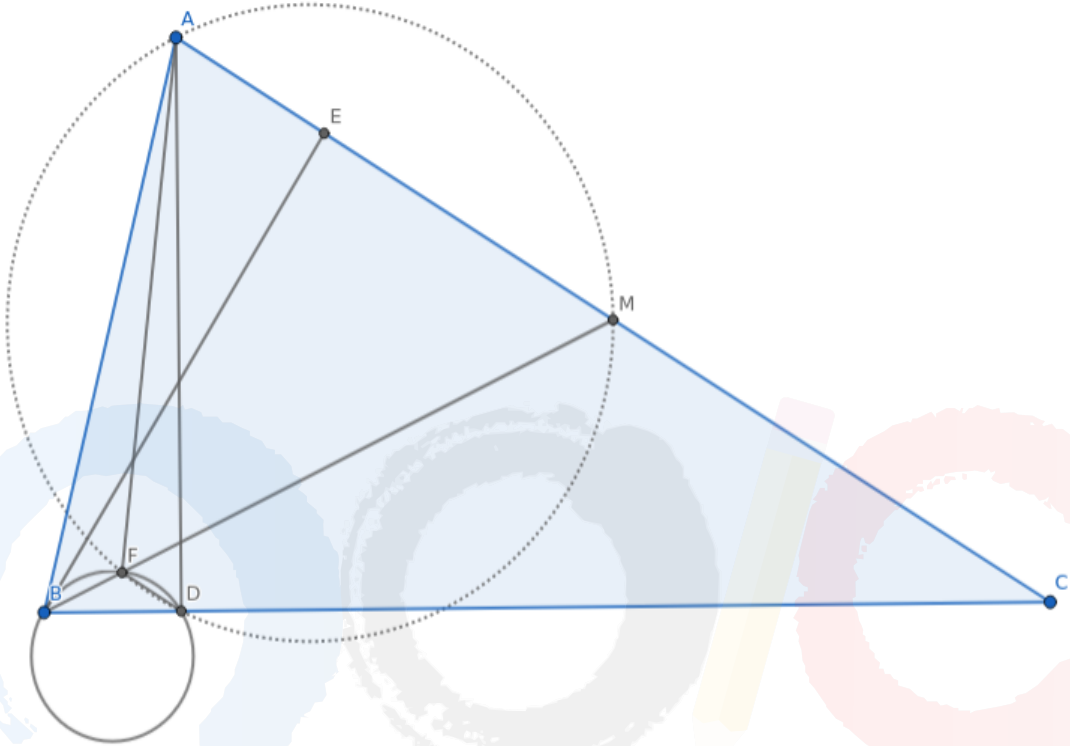
\includegraphics[width=0.5\textwidth]{first.png}
      \caption{Uma figura ilustrando a solução do terceiro problema. \href{https://noic.com.br/wp-content/uploads/2023/11/Solucoes_da_TM2_Nivel_A.pdf}{Fonte}}
    \end{figure}
    
    Dado:
    \[
      \angle DAC = \angle EBC = 90^\circ - \angle C \quad \text{e} \quad \angle EBC = \angle EBM + \angle MBC.
    \]

    Pelo \textit{teorema do segmento alterno}:
    \[
      \angle EBM = \angle FDB \Rightarrow \angle MFD = \angle FDB + \angle FBD = 90^\circ - \angle C,
    \]

    portanto, \( AFDM \) é um quadrilátero cíclico. Além disso:
    \[
      \angle DFM = \angle DAM \quad \text{e} \quad \angle AFM = \angle ADM.
    \]

    Como \( MD \) é mediana de \( \triangle ADC \), tem-se:
    \[
      MA = MD = MC \Rightarrow \triangle ADC \text{ é isósceles} \Rightarrow \angle MAD = \angle ADM.
    \]

    \clearpage

    \subsection{Problema 4.}
      \begin{tcolorbox}[problembox={Enunciado do problema}]
        Determine todos os inteiros positivos \( n \) para os quais existe um
        tabuleiro \( n \times n \), onde podemos escrever \( n \) vezes cada um dos
        números de \( 1 \) a \( n \) (um número em cada casa), de modo que as \( n \)
        somas dos números em cada linha deixem \( n \) restos distintos na divisão por
        \( n \), e as \( n \) somas dos números em cada coluna deixem \( n \) restos
        distintos na divisão por \( n \).
      \end{tcolorbox}

      Deve-se perceber que para todo $n$ ímpar, a configuração abaixo satisfaz o enunciado,
      mas nenhum $n$ par satisfaz tal.
  
      \begin{figure}[h]
        \centering
        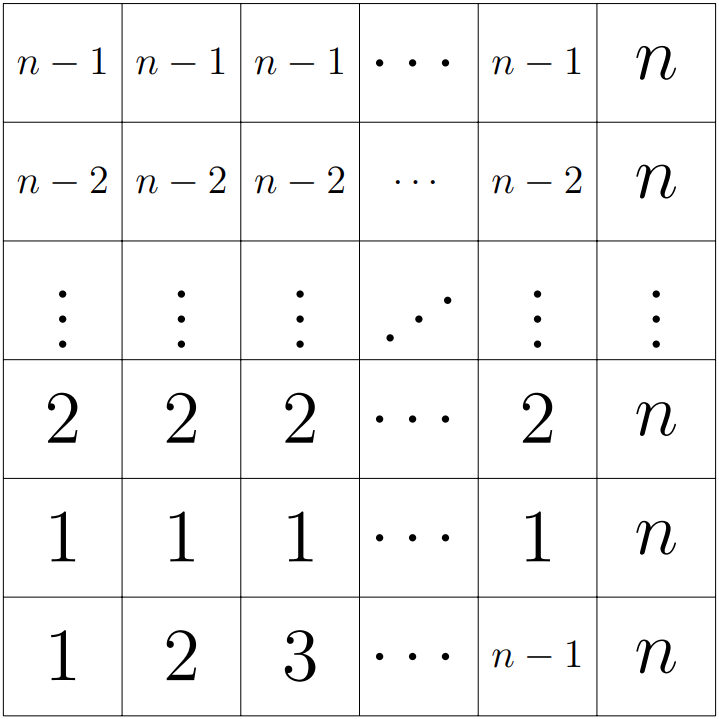
\includegraphics[width=0.35\textwidth]{second.png}
        \caption{Uma possível configuração para o quarto problema. \href{https://noic.com.br/wp-content/uploads/2023/11/Solucoes_da_TM2_Nivel_A.pdf}{Fonte.}}
      \end{figure}

      Para provar que todas as linhas têm somas diferentes $\pmod{n}$, deve-se perceber que,
      para quaisquer duas linhas distintas entre si e distintas entre a última linha, é
      possível achar este absurdo:
      \[
        x(n-1) + n \equiv y(n-1) + n \pmod{n} \Rightarrow x \equiv y \pmod{n}
      \]

      Já para qualquer linha distinta da última linha, é possível encontrar este outro 
      absurdo, já que n é um número ímpar e $\frac{n}{2}$ não é um inteiro:
      \[
        x(n-1) + n \equiv \frac{n(n+1)}{2} \pmod{n} \Rightarrow x \equiv \frac{n}{2} \pmod{n}
      \]

      Já para $n$ igual a um número par, a soma de todos os números no tabuleiro é igual
      a $\frac{n^2(n+1)}{2}$ e a soma de todos os números $\pmod{n}$ é igual a 
      $0 + 1 + 2 + ... + (n - 1) = \frac{n(n-1)}{2}$, logo:
      \[
        \frac{n^2(n+1)}{2} \equiv \frac{n(n-1)}{2} \pmod{n} \Rightarrow \frac{n(n^2+1)}{2} \equiv 0 \pmod{n}
      \]
      $n$ é par, logo $\frac{n}{2} \in \mathbb{Z}$. Logo, pode-se encontrar o absurdo
      abaixo, que anula a existência de um número $n$ par:
      \[
        \frac{n(n^2 + 1)}{2} \equiv \frac{n}{2} \equiv 0 \pmod{n}
      \]

  \clearpage

  \section{\textsf{Referências}}

    Só foi possível escrever este documento graças a ajuda e inspiração dos seguintes:

    \renewcommand{\refname}{\vspace{-2em}}
    \begin{thebibliography}{9}
      \bibitem{noic}
      NOIC - Núcleo Olímpico de Iniciação Científica.
      \textit{Soluções TM$^2$ Nível A}, 2023.
      Disponível em: \url{//noic.com.br/wp-content/uploads/2025/03/Solucoes_do_TM2_2024_Nivel_A.pdf}
    \end{thebibliography}
\end{document}

